\section{Архитектура решения}
\label{sec:Chapter1} \index{Chapter1}

\begin{figure}
    \centering
    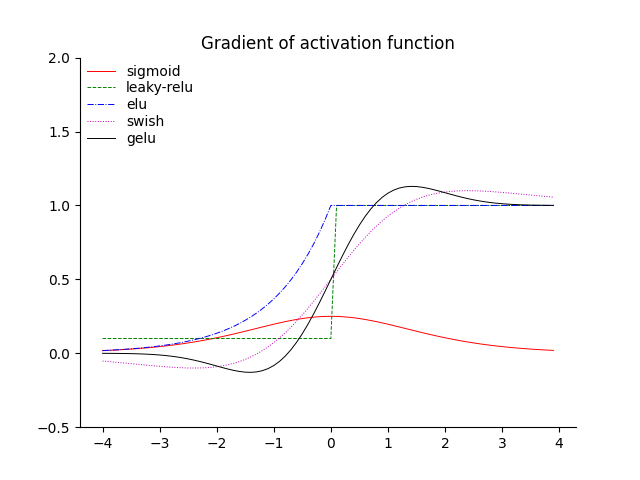
\includegraphics[scale=1]{./images/activation-funs-grad.png}
    \caption{\protect\hypertarget{image1}{Градиенты некоторых популярных функций активации.}}
\end{figure}


Современные модели, применяемые в задаче распознавания рукописного текста, обычно включают в себя три ключевых компонента:
\begin{enumerate}
\item Сверточную нейронную сеть, используемую для извлечения признаков из входных данных.
\item Последовательный энкодер
\item Декодер, который завершает процесс, трансформируя закодированные данные в окончательную текстовую транскрипцию с учетом информации, полученной от энкодера.
\end{enumerate}

\subsection{Извлечение визуальных признаков с помощью сверточной сети}
Подобно другим задачам компьютерного зрения, сверточная сеть используется для извлечения соответствующих визуальных признаков из текстовых изображений. Следующие архитектуры являются популярным выбором: ResNet \hyperlink{cite.Kai15}{[17]}, Inception \hyperlink{cite.Sze14}{[18]}, MobileNet \hyperlink{cite.San18}{[19]}. Увеличение сложности сверточной сети, как правило, приводит к умеренному приросту точности модели \hyperlink{cite.Her21}{[20]}. В этой работе используется архитектура ResNet. 

\newpage

\begin{figure}
    \centering
    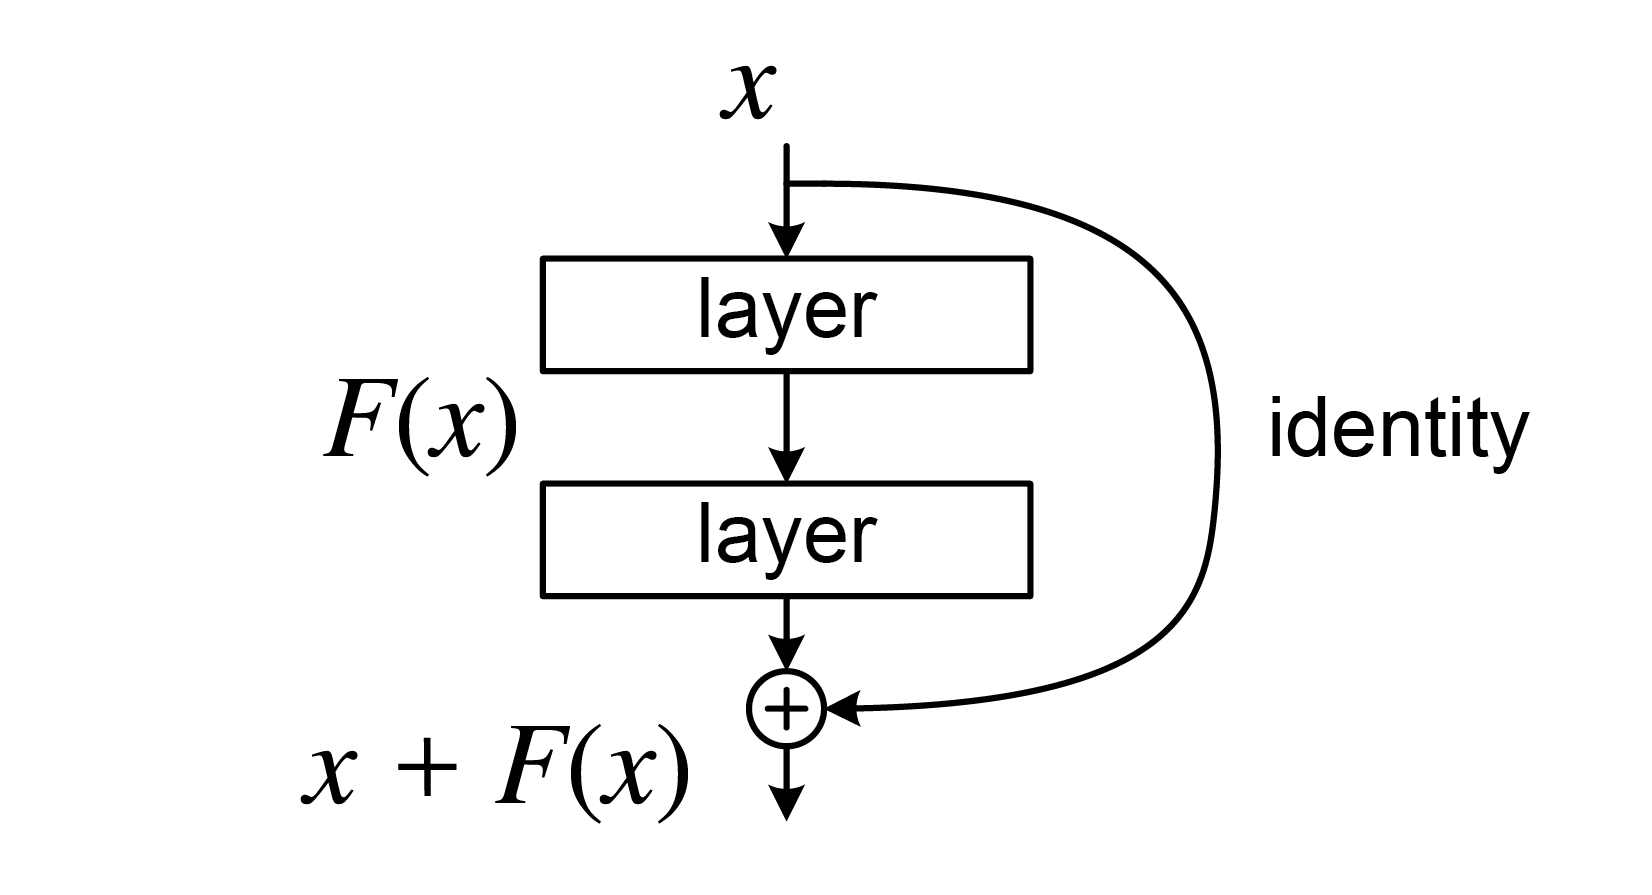
\includegraphics[scale=1]{./images/ResBlock.png}
    \caption{\protect\hypertarget{image2}{Residual блок.}}
\end{figure}

\subsubsection{Residual connection}
При обучении глубоких моделей градиент имеет тенденцию становиться очень маленьким: это называется проблема исчезающего градиента. Это связано с тем, что градиент проходит через ряд слоев, каждый из которых может уменьшить его. Например, градиент многих популярных функций активации приближается к нулю на значительной части числовой прямой \hyperlink{image1}{[Рис 1]}. 

Одним из решений проблемы исчезающего градиента является использование в качестве слоев нейронной сети residual блока \hyperlink{image2 }{[Рис 2]}, определенного следующим образом:
\begin{equation}
	\mathcal{F}_{l}^{'}(x) = \mathcal{F}_{l}(x) + x
\end{equation}
где $\mathcal{F}_{l}$ - стандартное нелинейное отображение (например, линейное - функция активации - линейное). Зачастую легче научиться предсказывать небольшое возмущение на входе, чем результат напрямую.

Модель с residual блоком имеет такое же количество параметров, как и модель без него, но ее легче тренировать. Причина в том, что градиенты могут перетекать непосредственно из выходных данных в более ранние слои. Чтобы убедиться в этом, рассмотрим градиент функции ошибки по параметрам слоя $l$. Имеем
\begin{equation}
	z_L = z_l + \sum_{i=l}^{L-1} \mathcal{F}_i(z_i ; \theta_i)
\end{equation}
где $z_i$ - признаки на выходе из $i$-го слоя сети. Таким образом, мы можем вычислить градиент функции потерь относительно параметров $l$-го слоя следующим образом:
\begin{equation}
	\frac{\partial \mathcal{L}}{\partial \theta_{l}} = 
	\frac{\partial z_{l}}{\partial \theta_{l}} \frac{\partial \mathcal{L}}{\partial z_{L}}
	(1 + \sum_{i=l}^{L-1} \frac{\partial \mathcal{F}_i(z_i; \theta_i)}{\partial z_{l}})
\end{equation}
Таким образом, мы видим, что градиент на слое $l$ напрямую зависит от градиента на слое $L$, причем независимо от глубины сети.
\begin{figure}
    \centering
    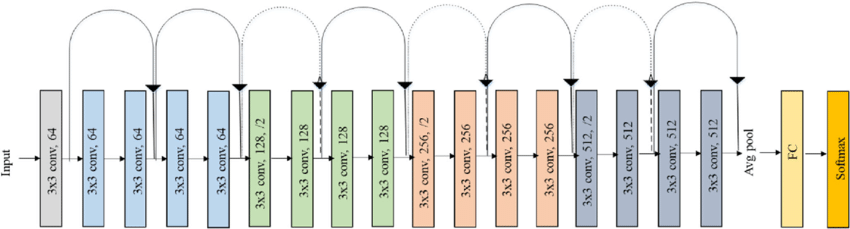
\includegraphics[scale=0.3]{./images/ResNet18.png}
    \caption{\protect\hypertarget{image3}{Архитектура ResNet-18.}}
\end{figure}

\newpage
\subsubsection{ResNet}
Победителем конкурса по компьютерному зрению \href{https://image-net.org/challenges/LSVRC/2015/}{ImageNet} 2015 года стала команда Microsoft, предложившая модель, известную сейчас как ResNet \hyperlink{image3}{[Рис 3]}. Данная модель состоит из residual блоков, имеющих следующий вид: свертка-BN-relu-свертка-BN, где BN - батч нормализация \hyperlink{cite.Iof15}{[21]}). Подобная архитектура позволяет обучать очень глубокие модели, а также решает проблему затухания градиентов. Именно из-за указанных преимуществ, а также из практического опыта, данная архитектура была отобрана для проведения данного исследования.

\begin{figure}
    \centering
    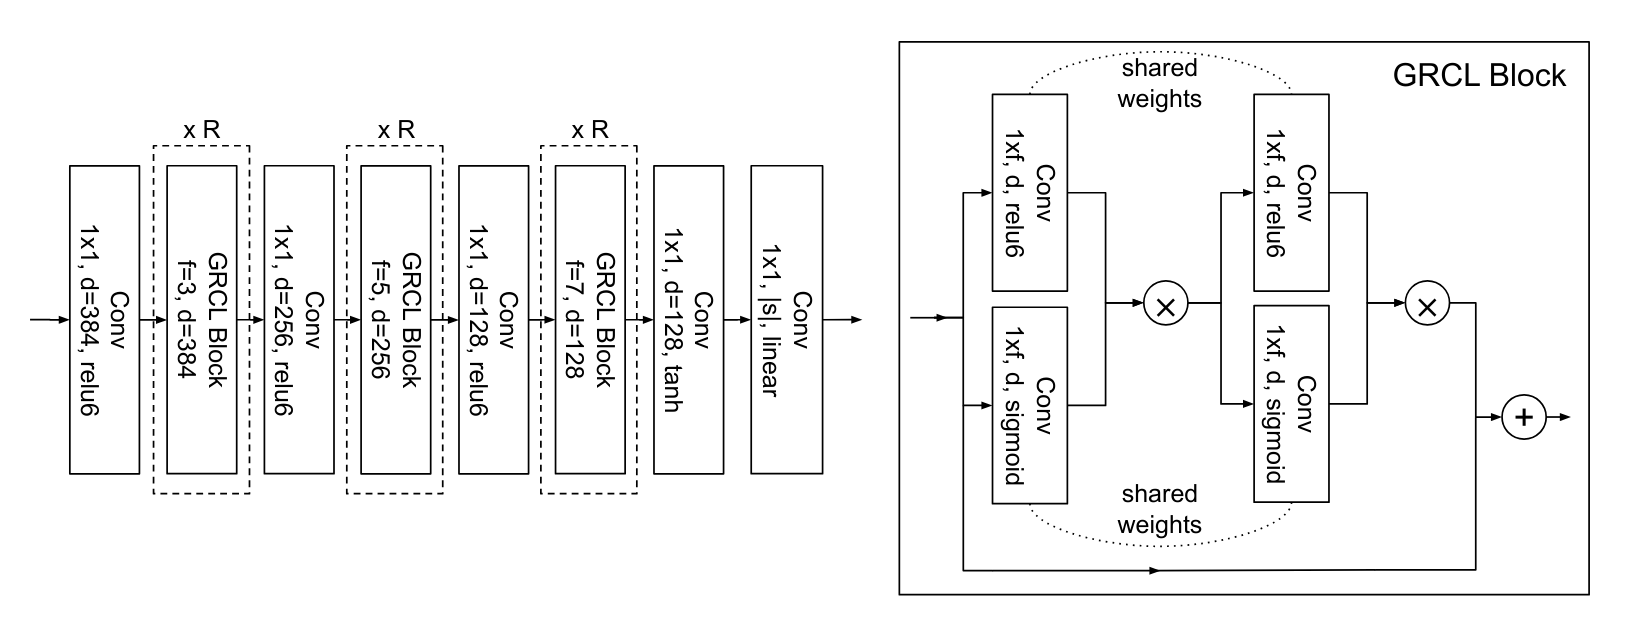
\includegraphics[scale=0.3]{./images/GRCL.png}
    \caption{\protect\hypertarget{image4}{Архитектура GRCL.}}
\end{figure}

\subsection{Последовательный энкодер}
Сверточная сеть, предназначенная для извлечения визуальных признаков, имеет ограниченное рецептивное поле, что ограничивает ее способность учитывать широкий контекст информации. Это создает сложности при обработке длинных последовательностей в сложных сценариях, таких как распознавание рукописного текста. Для учета контекста на больших расстояниях используется энкодер. Существует много различных
архитектур энкодера, далее будут рассмотрены основные из них.

\subsubsection{Рекуррентные нейронные сети}
Рекуррентная нейронная сеть — это нейронная сеть, которая отображает входное пространство последовательности в выходное пространство последовательностей с сохранением состояния. То есть элемент выходной последовательности $y_t$ зависит не только от элемента входной последовательности $x_t$, но и от скрытого состояния системы $h_t$, которое обновляется. Для простоты обозначений пусть T будет длиной вывода (с учетом того, что она выбирается динамически). Тогда рекурентная сеть соответствует следующей условной генеративной модели:

\begin{equation}
	p(y_{1:T} | x) = \sum_{h_{1:T}} p(y_{1:T}, h_{1:T} | x) = \sum_{h_{1:T}} \prod_{t=1}^{T} p(y_{t} | h_{t})p(h_{t} | h_{t-1}, y_{t-1}, x)
\end{equation}
где $h_t$ — скрытое состояние, и где мы определяем $p(h_1 |h_0, y_0, x) = p(h_1 |x)$ как начальное скрытое состояние. Мы предполагаем, что скрытое состояние вычисляется детерминированно следующим образом:

\begin{equation}
	p(h_t | h_{t-1}, y_{t-1}, x) = \mathbb{I}(h_t = f (h_{t-1}, y_{t-1}, x)) 
\end{equation}
для некоторой детерминированной функции $f$. Функция обновления $f$ обычно задается выражением

\begin{equation}
	h_t = \varphi (W_{xh} [x; y_{t-1}] + W_{hh}h_{t-1} + b_h) 
\end{equation}

Рекурентные сети с достаточным количеством скрытых единиц в принципе могут запоминать входные данные из далекого прошлого. Однако сети с "ванильной" архитектурой не могут этого сделать из-за проблемы исчезающего градиента. Существует архитектурное решение данной проблемы, в котором мы обновляем скрытое состояние аддитивным способом, аналогично residual блокам в ResNet: GRU и LSTM.

Различные варианты рекуррентных сетей использовались для решения задачи распознавания рукпоисного текста: LSTM \hyperlink{cite.Bas14}{[5]} \hyperlink{cite.Gra08}{[4]}, BiLSTM \hyperlink{cite.The17}{[6]} \hyperlink{cite.Joa17}{[7]}, Gated Recurrent Convolution Layer (GRCL) \hyperlink{image4}{[Рис 4]} \hyperlink{cite.Lux17}{[22]}.

\begin{figure}
    \centering
    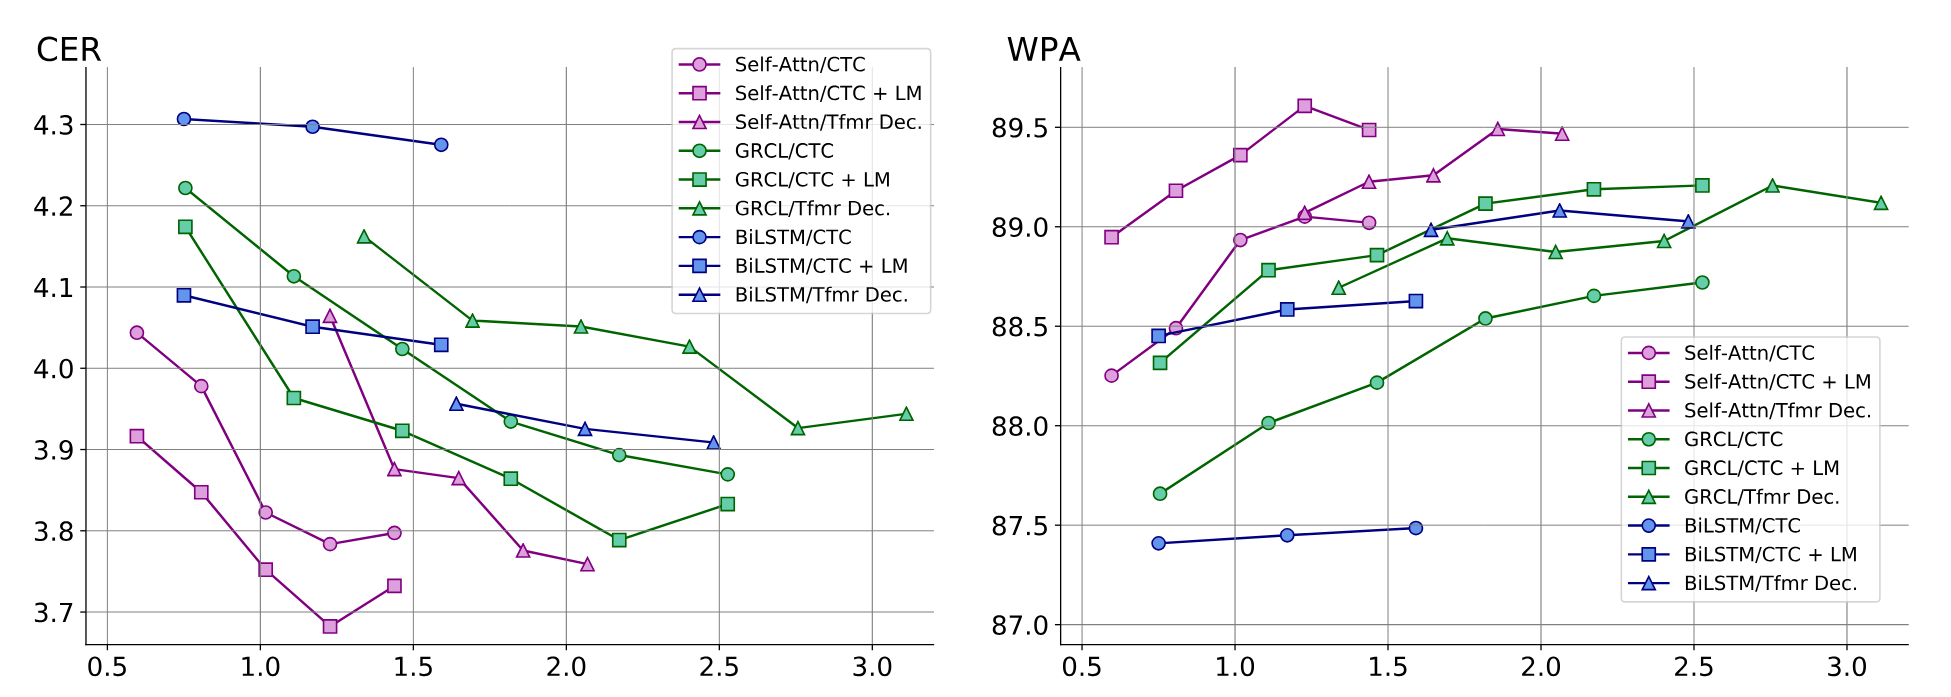
\includegraphics[scale=0.25]{./images/competition.png}
    \caption{\protect\hypertarget{image5}{Сравнение различных архитектур для задачи распознавания текста. \\ Взято из \protect\hyperlink{cite.Her21}{[20]}}.}
\end{figure}

\subsubsection{Self-Attention}
Self-Attention энкодер, предложенный в \hyperlink{cite.Vas17}{[3]} широко используется в задачах из NLP и компьютерного зрения. Распознавание текстовых строк, как задача преобразования изображения в последовательность, не является исключением. Self-attention способен улавливать долгосрочные зависимости в последовательностях лучше, чем рекуррентные сети, благодаря возможности обрабатывать взаимодействия между всеми элементами последовательности одновременно. Также, в отличие от рекуррентных сетей, self-attention не сталкивается с проблемой затухания градиентов.

Выход сверточной сети, с удаленным измерением высоты изображения ($X \in \mathbb{R} ^ {n \times d}$), поступает в энкодер. Выход $Y$ слоя Attention получается следующим образом:

\begin{equation}
\begin{split}
	Q = X W_q \\
	K = X W_k \\
	V = X W_v \\
	Y = softmax(\frac{Q K^T}{\sqrt{d}}V)
\end{split}
\end{equation}
где $W_q$, $W_k$ и $W_v$ — матрицы параметров размера $d \times d$, которые задают проекцию входной последовательности $X$ в пространство запросов, ключей и значений соответственно. Закодированный признак Y представляет собой выпуклую комбинацию вычисленных значений $V$, матрица  сходства вычисляется как скалярное произведение запросов и ключей.

Эффективность "ванильного" Attention может быть низкой, поскольку данный слой инвариантен к перестановкам, и, следовательно, игнорирует порядок элементов входной последовательности. Чтобы преодолеть эту проблему, к признакам элементов входной последовательности добавлятся информация о позиции элемента (positional embedding). Можно представить positional embedding как матрицу $\mathbf{P}^{n \times d}$.

В \hyperlink{cite.Vas17}{[3]} было предложено использовать синусоидальный базис следующего вида:
\begin{equation}
	p_{i,2j} = \sin(\frac{i}{C^{\frac{2j}{d}}}), \quad p_{i,2j+1} = \cos(\frac{i}{C^{\frac{2j}{d}}}) 
\end{equation}
где $C$ соответствует некоторой максимальной длине последовательности. Одним из важных плюсов данного представления является то, что представление одной позиции линейно предсказуемо относительно любой другой, если известно их относительное расстояние. В частности, выполняется $p_{t+ \phi} = f (p_t)$, где $f$ - некоторое линейное отображение. А именно
\begin{equation}
\begin{pmatrix}
	\sin(\omega_k (t + \phi)) \\
	\cos(\omega_k (t + \phi))
\end{pmatrix} = 
\begin{pmatrix}
	\cos (\omega_k \phi)  & \sin (\omega_k \phi) \\
	-\sin (\omega_k \phi) & \cos (\omega_k \phi)
\end{pmatrix}
\begin{pmatrix}
	\sin(\omega_k t) \\
	\cos(\omega_k t)
\end{pmatrix}
\end{equation}
То есть при маленьком $\phi$ имеем $p_{t + \phi} \approx p_t$. Positional embedding, как правило, прибавляется ко входу, то есть:
$PosEmbed(X) = X + \mathbf{P}$.

Существуют также другие варианты. Например, relative positional embedding \hyperlink{cite.Sha18}{[23]}.

\subsection{Декодер}
Декодеры берут признаки закодированной последовательности и пытаются декодировать ее текстовое содержимое. Архитектуры декодеров для рекурентных сетей были описаны ранее. Два других популярных подхода к решению этой задачи: transformer \hyperlink{cite.Vas17}{[3]} и Connectionist Temporal Classification \hyperlink{cite.Gra06}{[2]} декодеры.

\subsubsection{Transformer}
Декодер Transformer стал предпочтительным декодером для задач прогнозирования последовательности, таких как машинный перевод. Он также широко применяется в задаче распознавания рукописного текста. Например, state-of-the-art решение согласно бенчмарку \href{https://paperswithcode.com/sota/handwritten-text-recognition-on-iam}{IAM} принадлежит на момент написания этого текста decoder-only transformer архитектуре \hyperlink{cite.Mas23}{[8]}. Минус данной архитектуры - это то, что она является более громоздкой. Она требует большего количества параметров и, соотвественно, данных для обучения \hyperlink{image5}{[Рис 5]}.

\begin{figure}
    \centering
    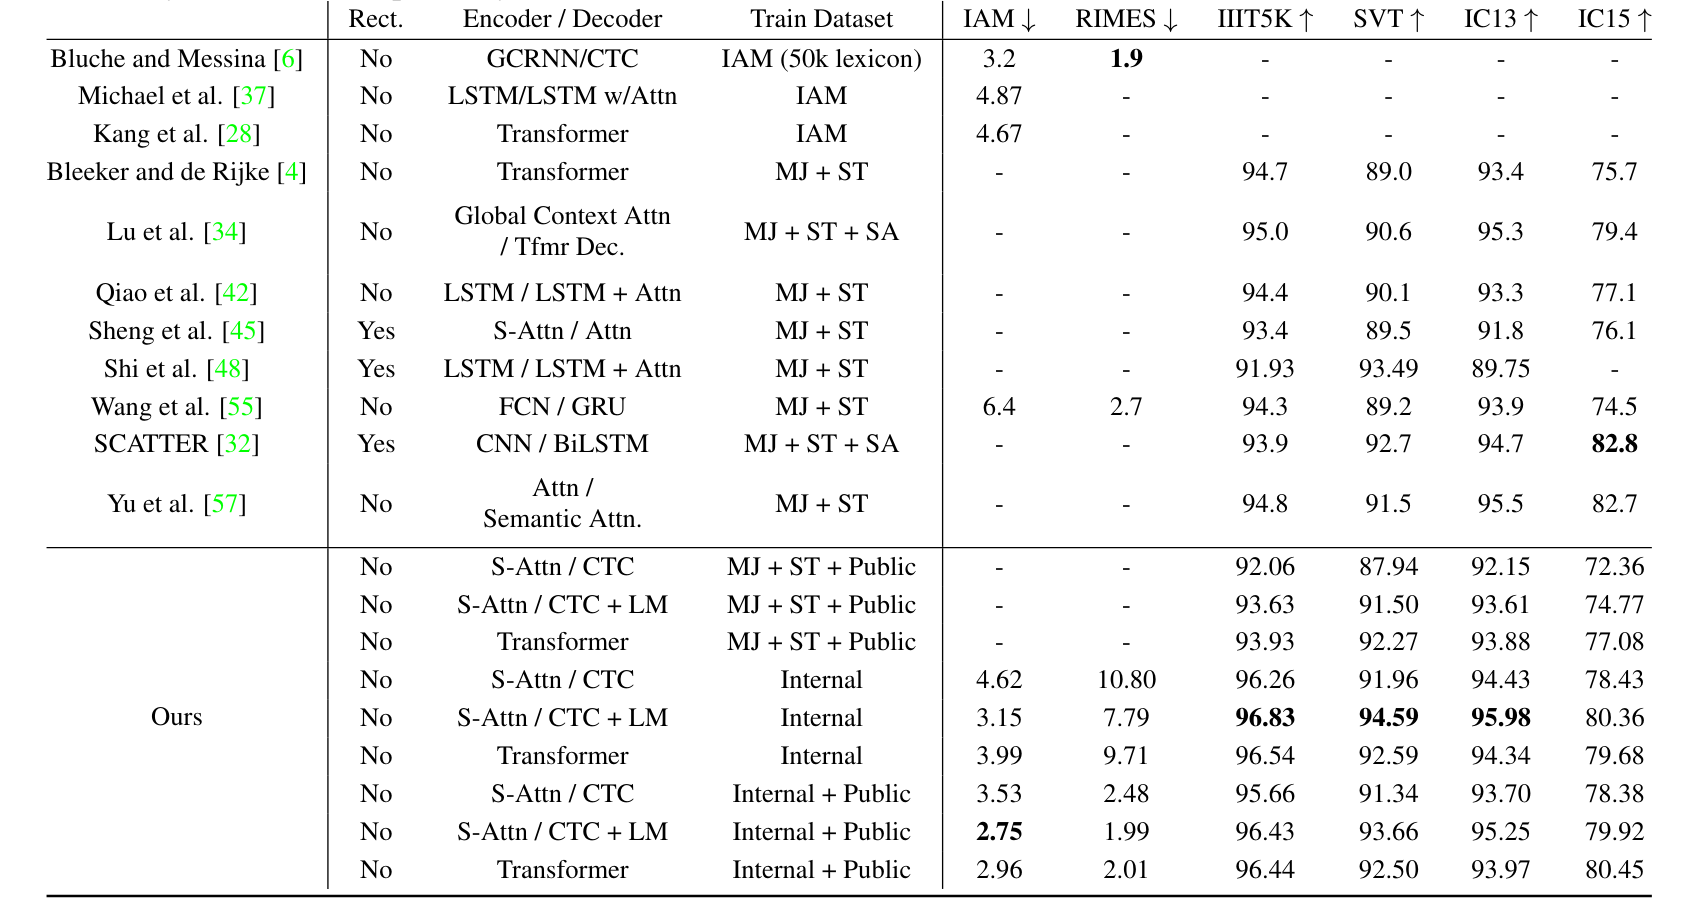
\includegraphics[scale=0.25]{./images/competition_all.png}
    \caption{\protect\hypertarget{image6}{Сравнение различных архитектур для задачи распознавания текста на различных бенмарках. \\ Взято из \protect\hyperlink{cite.Her21}{[20]}}.}
\end{figure}

\subsubsection{Connectionist Temporal Classification}
Декодер Connectionist Temporal Classification изначально использовался для распознавания речи, позже исследователи добились огромного успеха, применив его для задач распознавания текста. Далее представлен математический формализм временной классификации, а также ошибки, используемой в качестве метрики в данном исследовании.

Пусть S - это набор обучающих примеров, выбранных из фиксированного распределения $D_{\mathcal{X} \times \mathcal{Z}}$. Пространство входных данных $\mathcal{X} = (\mathbb{R}^m)^*$ представляет собой множество всех последовательностей из m-мерных векторов вещественных чисел. Целевое пространство $\mathcal{Z} = L^*$ представляет собой множество всех последовательностей из (конечного) алфавита $L$. В общем случае, мы обозначаем элементы $L^*$ как последовательности символов. Каждый пример в S состоит из пары последовательностей $(x, z)$. Целевая последовательность $z = (z_1, z_2, ..., z_U)$ не длиннее входной последовательности $x = (x_1, x_2, ..., x_T)$, то есть $U \leq T$. Поскольку входные и целевые последовательности обычно не имеют одинаковой длины, нет априорного способа их выравнивания.

Цель состоит в использовании $S$ для обучения временного классификатора $h : \mathcal{X} \rightarrow \mathcal{Z}$, который классифицирует ранее не виденные входные последовательности таким образом, чтобы минимизировать некоторую специфическую ошибку задачи.

Общепризнанным выбором является следующая ошибка: для заданного тестового набора $S_0 \subset D_{\mathcal{X} \times \mathcal{Z}}$, не пересекающегося с $S$, определяется коэффициент ошибок меток (label error rate, LER) временного классификатора $h$ как нормализованное расстояние Левенштейна между его предсказаниями и ответом на $S_0$, т.е.:
\begin{equation}
	LER(h, S_0) = \frac{\sum_{(x,z) \in S_0} ED(h(x), z)}{\sum_{(x,z) \in S_0} |z|}
\end{equation}
где $ED(p, q)$ - расстояние Левенштейна между двумя последовательностями $p$ и $q$, т.е. минимальное количество вставок, замен и удалений, необходимых для преобразования $p$ в $q$.
Это естественная метрика для задач (таких как распознавание речи или рукописного текста), где целью является минимизация частоты ошибок транскрипции. Популярными метриками в задаче распознавания рукописного текста являются WER (word error rate) и CER (character error rate) - описанное выше расстояние Левенштейна на уровне слов и символов соответственно.

Также в данном исследовании будет использоваться метрика LabelAccuracy (Label может быть словом, строкой или фрагментом). Определяется она так:
\begin{equation}
	LabelAcc(h, S_0) = 1 - LER(h, S_0)
\end{equation}


Пусть мы имеем некоторую нейронную сеть $N_w : (\mathbb{R}^m)^T \rightarrow (\mathbb{R}^n)^T$. Пусть $y = N_w(x)$ - последовательность выходов сети, и обозначим $y_t^k$ активацию выходного узла $k$ в момент времени $t$ (последний слой softmax). Тогда $y_t^k$ интерпретируется как вероятность наблюдения символа $k$ в момент времени $t$, что определяет распределение над множеством $L_{0}^T$ длины $T$ последовательностей алфавита $L_0 = L \cup \{blank\}$. Тут мы добавляем в алфавит символ $blank$, обозначающий пропуск. Элементы $L_0^T$ обычно называют путями.

\begin{equation}
	p(\pi|x) = \prod_{t=1}^{T} y_t^{\pi_t}, \quad \forall \pi \in L_{0}^{T}
\end{equation}

Далее определим отображение $B: L_{0}^T \rightarrow L_{\leq T}$, где $L_{\leq T}$ - это множество последовательностей длиной менее или равной $T$ по оригинальному алфавиту $L$. Мы делаем это, просто удаляя все пробелы и повторяющиеся символы из путей. Интуитивно это соответствует выводу нового символа, когда сеть переходит от предсказания отсутствия символа к предсказанию символа, или от предсказания одного символа к другому. Наконец, используем $B$ для определения условной вероятности данного предсказания $I \in L_{\leq T}$ как сумму вероятностей всех путей, соответствующих ему:
\begin{equation}
	p(I|x) = \sum_{\pi \in B^{-1}(I)} p(\pi|x)
\end{equation}

Вывод классификатора должен быть наиболее вероятным предсказанием для входной последовательности:
\begin{equation}
	h(x) = \arg\max_{I \in L_{\leq T}} p(I|x)
\end{equation}

В данном исследовании поиск такого предсказания строится на предположении, что наиболее вероятный путь будет соответствовать наиболее вероятному предсказанию:
\begin{equation}
\begin{split}
	h(x) \approx B(\pi^{*}) \\
	\pi^{*} = \arg\max_{\pi \in L_0^T} p(\pi|x).
\end{split}
\end{equation}
Это легко найти, так как $\pi^{*}$ представляет собой просто конкатенацию самых вероятных символов на каждом этапе. Такой подход не гарантирует нахождение наиболее вероятного предсказания, но достаточно хорошо его приблежает. 

Модель обучается методом максимального правдоподобия. Для вычисления условных вероятностей $p(I|x)$ отдельных предсказаний используется динамическое программирование \hyperlink{cite.Gra06}{[2]}. Также включение явной языковой модели поверх логитов может значительно повысить точность \hyperlink{cite.Fuj17}{[24]}.
\paragraph{}
Во время выбора архитектуры учитывался собственный практический опыт, а также результаты исследований по данной теме. Например, в \hyperlink{cite.Her21}{[20]} проводится сравнительный анализ различных архитектур энкодеров / декодеров \hyperlink{image6}{[Рис 6]}. Было решено выбрать в качестве:
\begin{enumerate}
\item Сверточной нейронной сети: ResNet
\item Последовательного энкодера: TransformerEncoder
\item Декодера: Connectionist Temporal Classification
\end{enumerate}

\newpage